\section{Design og implementering}\label{sec:filter_design}
For at kunne implementere anti-alias lav pas filtrene i praksis blev det valgt at designe et 
prototype print hertil. Da printet blev designet i starten af projektets forløb hvor filteret 
endnu ikke var færdig dimensioneret, blev det valgt at designe et generisk Sallen-Key biquad 
der kan anvendes til alle de fire, i litteraturen opgivet, designmetoder. Kredsløbet kan ses i 
figur \ref{fig:skbiquadsch}.



\begin{figure}[H]
	\centering
	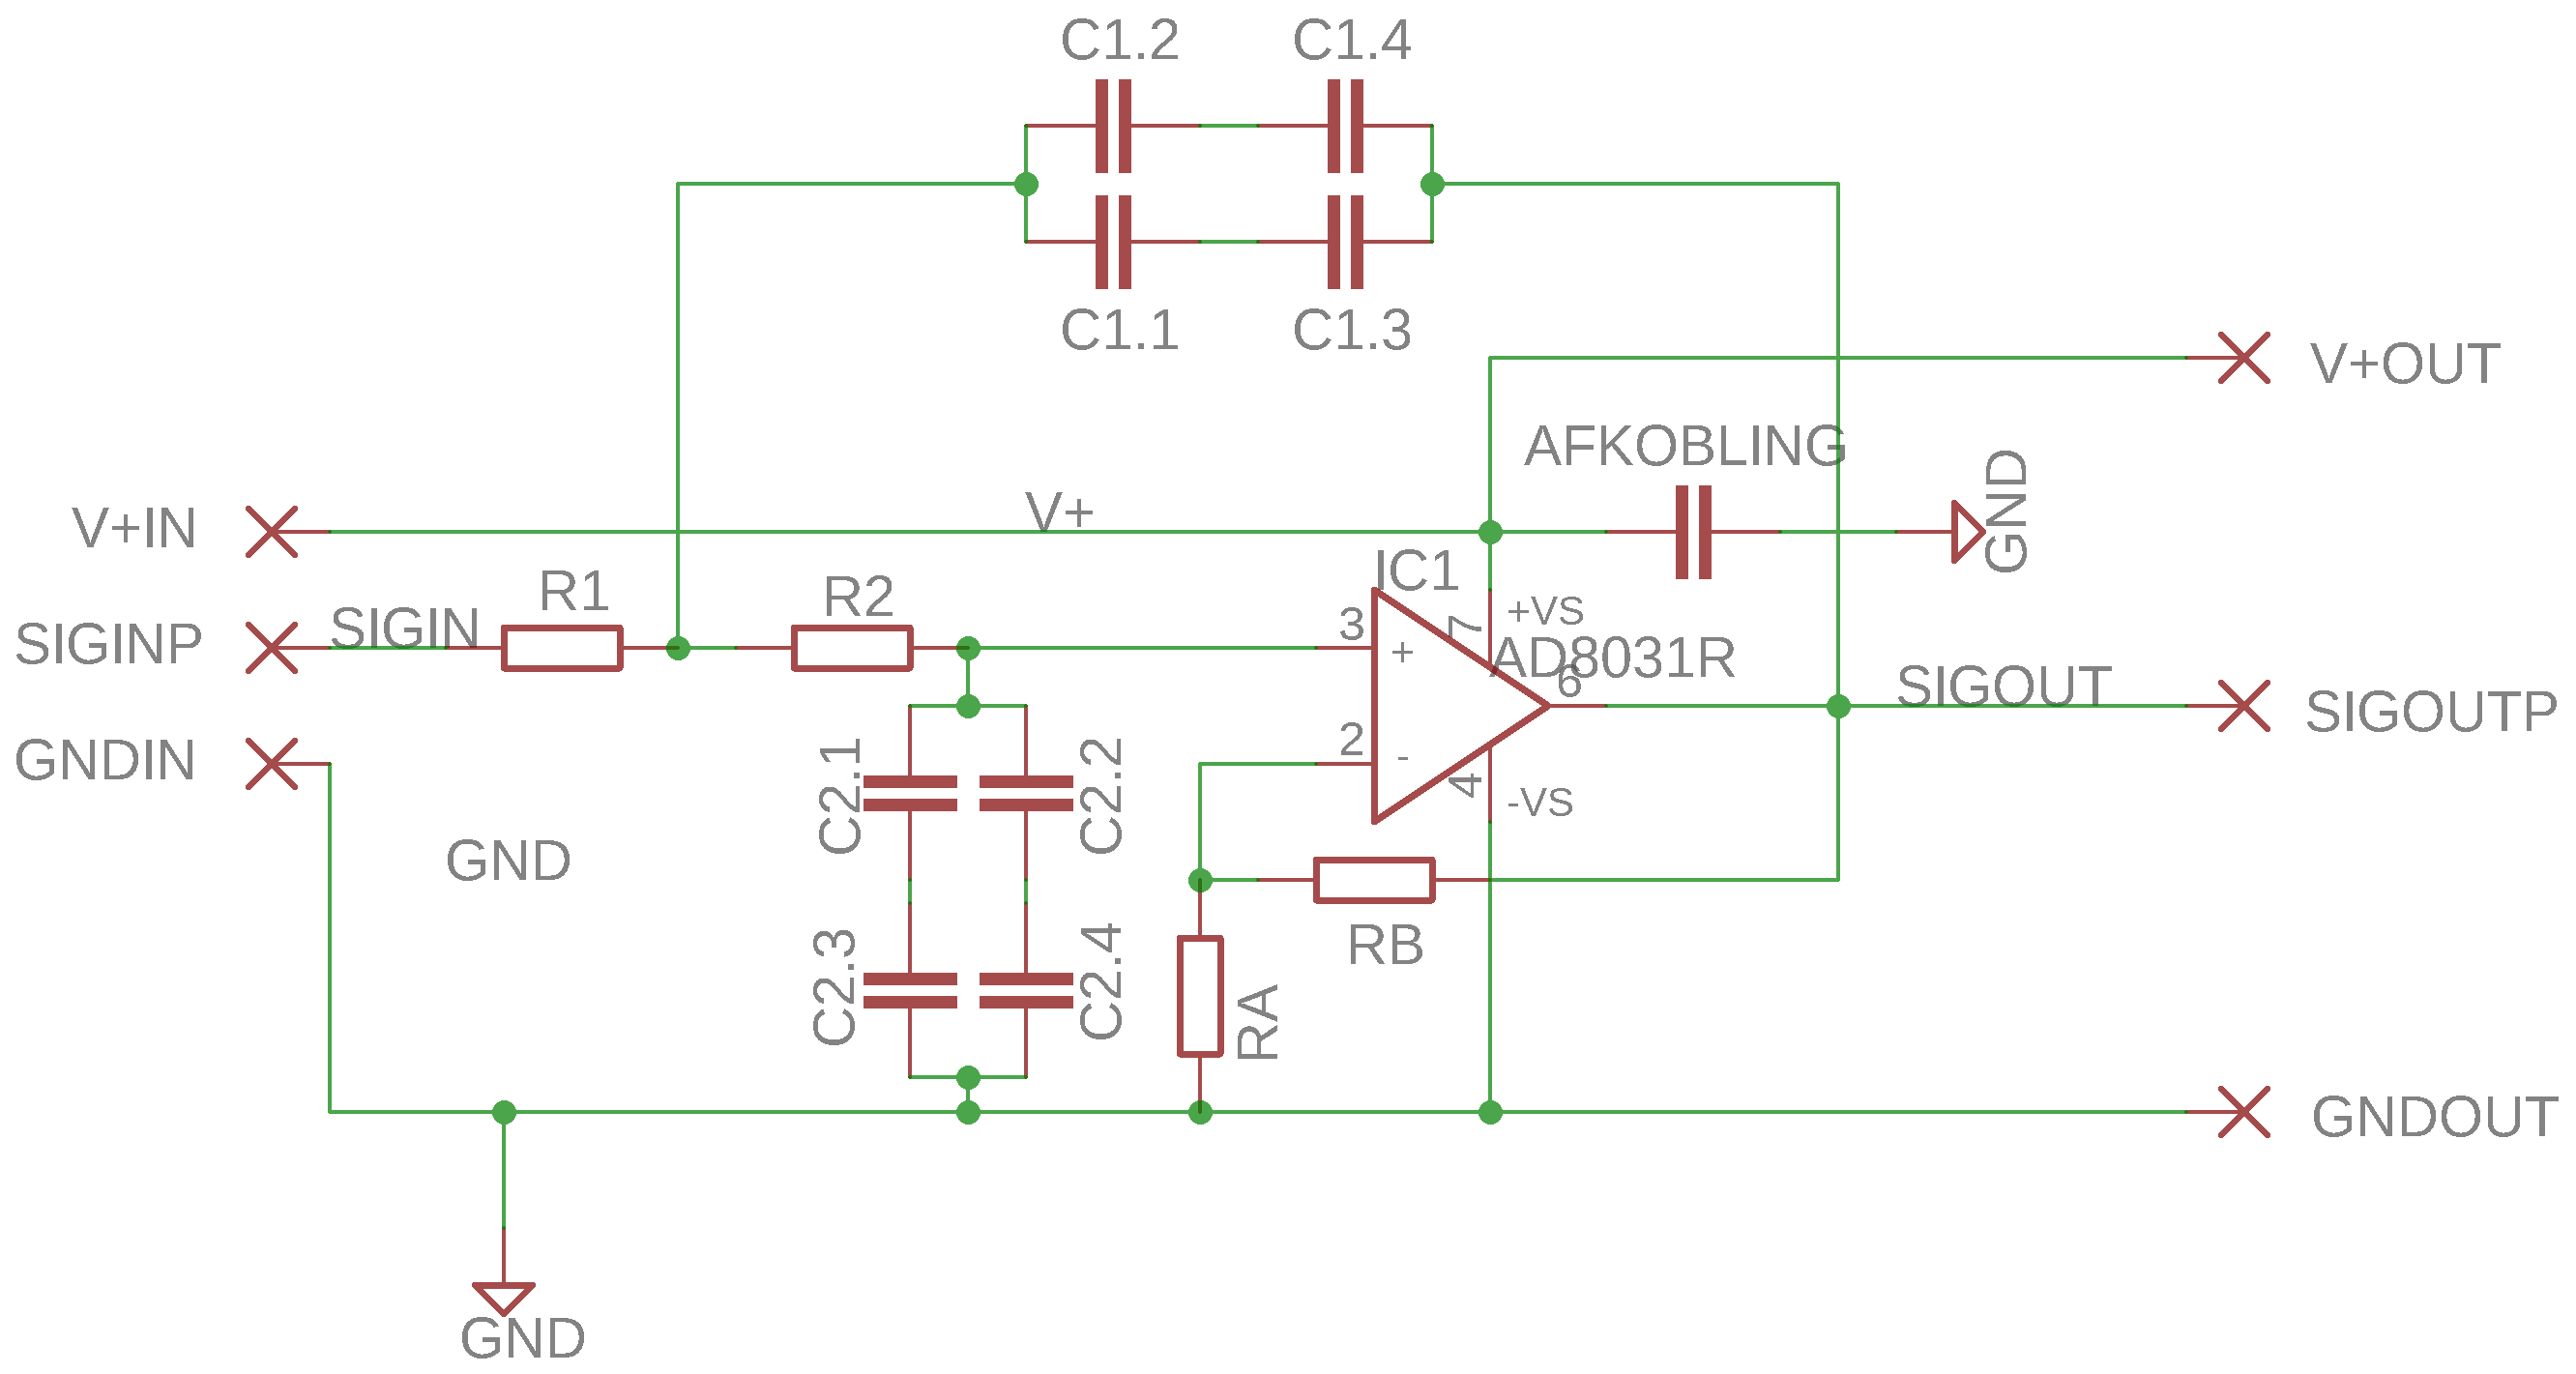
\includegraphics[width=.7\linewidth]{billeder/skbiquadsch}
	\caption{Lav pas biquad prototype kredsløb}
	\label{fig:skbiquadsch}
\end{figure}

Som det kan ses på figuren så er begge kondensatorer erstattet med en parallelforbindelse af 
to serie forbundne kondensatorer. Dette valg gør at det langt nemmere at opnå en specific 
kapacitans, ved at anvende op til fire kondensatorer fra rækken af værdier der er tilgængelig.

Disse kondensatorer blev beregnet ved at lave et matlab script som finder alle mulige kombinationer, for de kondensatorer som var tilgængelig på SDU under projektets udførelse.

Som det kan ses i tabel \ref{tab:kapvskap} bliver den faktiske kapacitans rigtig tæt på den
beregnede, dog er der her ikke taget højde for usikkerheden i komponentværdierne.

\begin{table}[h!]
	\centering
	\caption{Beregnede kondensatorer og tætteste mulige kombinationer serie/parallel}
	\begin{threeparttable}
		\begin{tabular}{l c c c c}
			\toprule
			& \multicolumn{2}{c}{\textbf{Beregnede værdier}} & \multicolumn{2}{c}{\textbf{Tætteste mulige kombinationer}} \\ 
			\midrule
			\textbf{Filter \#} &
			\textbf{$C_{1}$} 	& 
			\textbf{$C_{2}$}  	&
			\textbf{$C_{1}$} 		& 
			\textbf{$C_{2}$} 	\\
			\midrule
			1 & \num{2.2573E-09}\farad & \num{1,5703E-09}\farad & \num{2.2585e-09}\farad & \num{1.57e-09}\farad \\
			
			2 & \num{3,0832E-09}\farad & \num{4,3476E-10}\farad & \num{3.08073e-09}\farad & \num{4.3477e-10}\farad \\
			
			3 & \num{8,4273E-09}\farad & \num{9,8146E-11}\farad & \num{8.4259e-09}\farad & \num{9.8409e-11}\farad \\
			\bottomrule
		\end{tabular}
	\end{threeparttable}
\label{tab:kapvskap}
\end{table}

Det valgtes at lave hver bi-quad som et separat print der kan kobles sammen med et lignende
sig selv. 
Dette giver de fordele at det vil forekomme nemmere at fejlfinde på de enkelte led, og
samtidigt kan der laves flere forskellige ordener af filtret uden at skulle ændre på PCB designet.

Det færdige PCB design kan ses på figur \ref{fig:skbiquadpcb}. Her kortsluttes RB, og RA forbliver ikke forbundet, og så påsættes der selvfølgelig de beregnede komponenter for at opnå det specificerede filter bi-quad. 

is man sammenligner resultaterne fra testen i bilag 
\ref{sec:test_aafilter} med den beregnede filter karakteristik vist i figur 
\ref{fig:filter_cheb1_denorm}, kan det ses at filteret i pasbåndet har en konstant dæmpning
på ca. $3\si\decibel$. Denne dæmpning er senere fundet til at være pga. en for stor indgangs spænding under forsøget, hvilket har ført til at operationsforstærkerne i filteret er gået i mætning, der har dog ikke været tid til at lave nye målinger.
Dette kan der dog ses bort fra da karakteristikken ellers er korrekt bortset fra en forskydning på $3\si\decibel$. 
\hlh{Måske dette skal føres til en delkonklusion i kapitlet??}
Udover dette kan det ellers konkluderes at implementeringen af filteret overholder designet,
da både knækfrekvensen og hældningen i mellem pas og stop bånd stemmer overens.


\begin{figure}[H]
	\centering
	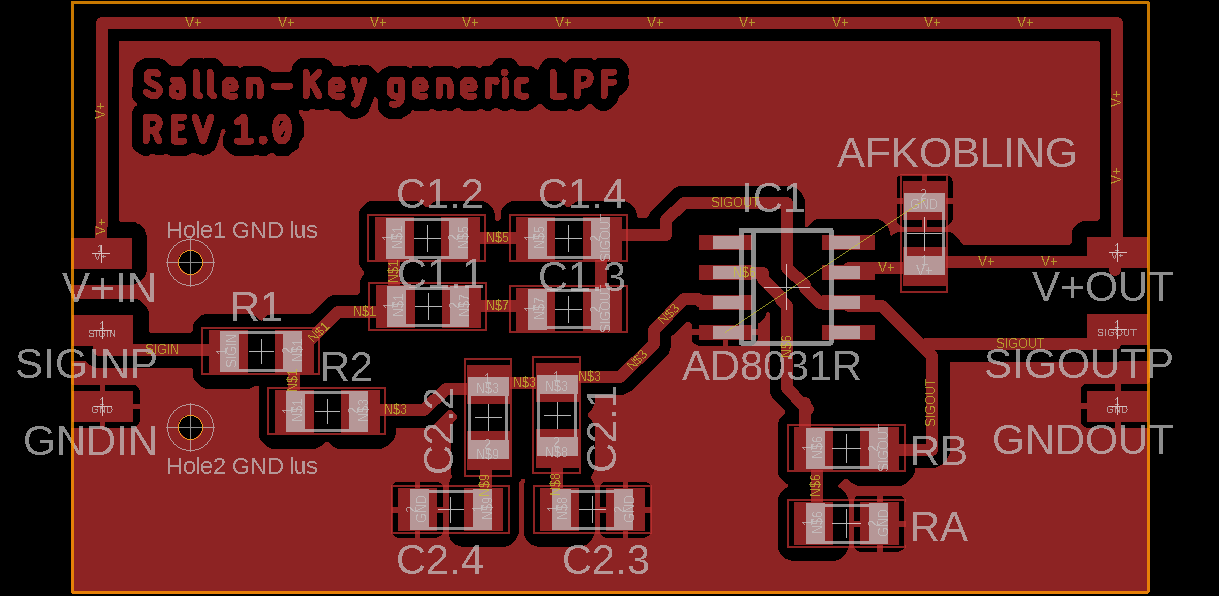
\includegraphics[width=.7\linewidth]{billeder/skbiquadpcb}
	\caption{Lav pas biquad prototype PCB design}
	\label{fig:skbiquadpcb}
\end{figure}

\section{Rekonstruktions filter}

Når signalet skal genskabes efter behandling i mikroprocessoren gøres dette ved hjælp af en DAC (Digital to Analog Converter). 
Måden denne virker på er ved at anvende et så kaldt sample-and-hold kredsløb,
dette betyder at værdien der skal genskabes bliver sat og holdt i en
tidsperiode ($T=\frac{1}{f_s}$), dette skaber en række firkant pulser som
illustreret til venstre i figur \ref{fig:samplholdrecon}.

Her skabes dog så en masse højfrekvente komponenter som er uønskede, disse dele af signalet kan så filtreres fra, og derved "udglatte" signalet, ved at anvende et rekonstruktions lav-pas filter.

I praksis anvendes oftes det samme filter signal som anti-aliasing filteret,
så længe at sampling frekvensen er konstant og bit opløsningen på DAC og ADC
er ens. Dette er muligt da det rekonstruerede signal er i det samme frekvens
spektrum som det der samples.

Til dette projekt er der også anvendt det samme filter design, til både anti-aliasing og rekonstruktions filteret.

\begin{figure}[H]
	\centering
	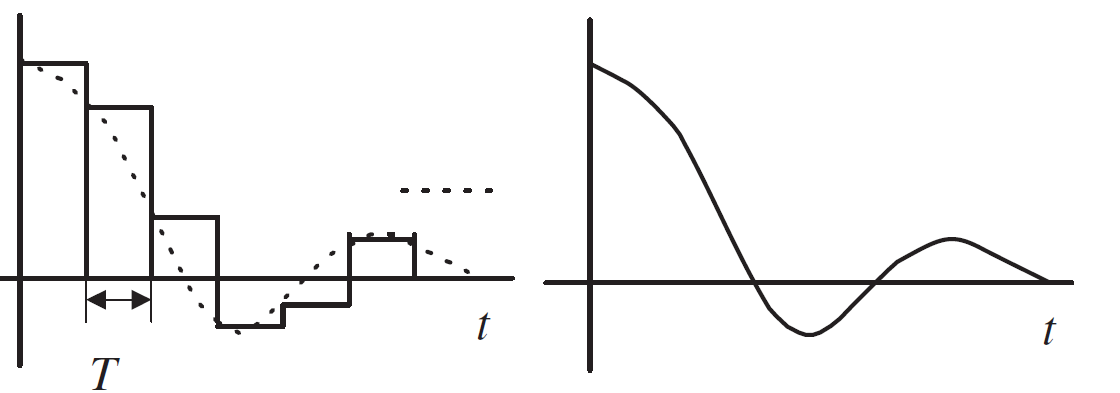
\includegraphics[width=0.6\linewidth]{billeder/dacrecon}
	\caption{Udgang fra DAC med sample-and-hold, før og efter rekonstruktionsfilter. Kilde:\cite{Tan2013}}
	\label{fig:samplholdrecon}
\end{figure}
